% !TeX root = ../main.tex

%%%%%%%%%%%%%%%%%%%%%%%%%%%%%%%%%%%%%%%%%%%%%%%%%%%%%%%%%%%%%%%%%%%%%%%%%%%%%%%%%%
%%																				%%
%% File name: 		body.tex													%%
%% Project name:	Applications in Deep Learning								%%
%% Type of work:	Advanced Seminar											%%
%% Author:			Hannes Bohnengel											%%
%% Mentor:			Debayan Roy													%%
%% Date:			09 June 2017												%%
%% University:		Technical University of Munich								%%
%% Comments:		Created in texstudio with tab width = 4						%%
%%																				%%
%%%%%%%%%%%%%%%%%%%%%%%%%%%%%%%%%%%%%%%%%%%%%%%%%%%%%%%%%%%%%%%%%%%%%%%%%%%%%%%%%%

\section{Conventional Speech Synthesis}
\label{sec:speech}

\textbf{\color{ACMRed}Short text with content of this chapter}

\subsection{Motivation \& Approaches}
\label{subsec:convenspeech}

Speech synthesis has emerged over the last 10 years due to a vast contribution by the global community of researchers and the increasing computational power for data processing. Its quality and naturalness has increased steadily and different approaches have been developed so far \cite{suendermann:challenges}. The typical applications like navigation systems in cars or telephone-based dialogue systems are nowadays widely established. But also as reading aid for visually impaired people \cite{readspeaker:tts} or as in the case of the famous scientist Stephen Hawking, who has been using a synthesized voice to communicate since 1997 \cite{hawking:speech}, speech synthesis has proven to be very useful. Another very interesting application of speech synthesis is shown in [XX]. The author proposed to introduce synthetic speech as means of communication between pilots, since there have been many accidents due to misunderstandings at radio-based communication. %Finally the interaction between man and machines or robots \cite{hill:manmachine}

According to \cite{hinterleitner:quality} speech synthesis can be divided into three types: Canned speech, \ac{CTS} and \ac{TTS}. Canned speech more or less is the play back of prerecorded spoken sentences or words with none or very little adjustments. A typical example are the announcements on train stations. Because of the high effort of recording everything (almost) exactly as it is played back, this approach is limited to only a few simple applications. With \ac{CTS} the waveform is generated out of a linguistic description without any information of the respective text. In this way no natural language processing is required, but nevertheless \ac{CTS} nowadays has not made any important impact. The last and most promising type is \ac{TTS}.

A \ac{TTS} system consists of a \ac{NLP} part, where the text is analyzed and the word and sentence structure and accents are extracted. In the next step these accents are used to generate the prosody of the given text like duration, intensity and pitch. Then the created phonetic representations with prosody information are stringed together to a continuous stream of signal parameters. The last task, the speech generation, uses this stream to generate the respective waveform. This function block can be implemented in different ways. In \cite{hinterleitner:quality} three general approaches are named as follows: Parametric Speech Synthesis (formant-based synthesis), Concatenative Speech Synthesis (unit-selection synthesis) and Statistical Parametric Speech Synthesis (\ac{HMM}-based synthesis). The methods in brackets are the respective implementations, which are most commonly used. 

The formant-based synthesis is the oldest approach. To generate a voice waveform, an excitation signal is fed into multiple formant filters which describe the characteristics of the human vocal tract. The output of the filters then forms the voice waveform. This technique is the only one which does not need any recorded speech, but instead generates the synthesized voice only by modeling the human vocal tract. The quality of the generated voice is the lowest in comparison to the other techniques, but therefore formant-based synthesizer have the smallest footprint and the voice characteristics can easily been modified by just changing the filter parameters~\cite{hinterleitner:quality}.

With the development of concatenative speech synthesizer the quality of the generated speech improved tremendously. Very similar to \ac{CTS} prerecorded speech is used as reference. Very basically said, the recorded speech is divided into units and these units are then stringed together to form the new speech signal according to a given text. Hereby the chosen size of the units determines both the footprint size and the voice quality. With larger units a higher voice quality can be achieved, but this also results in a much larger database. The challenge in unit-selection is to ensure, that the transissions between the units are as natural as possible~\cite{hinterleitner:quality}. In Section~\ref{subsec:hmmspeech} some concepts on how to achieve this as well as the third implementation, the \ac{HMM}-based synthesis, a specific instance of \ac{SPSS} are described in detail.

\subsection{\ac{HMM}-based Speech Synthesis}
\label{subsec:hmmspeech}

In this section the \ac{HMM}-based, the most recent approach for speech synthesis will be described further and both advantages and drawbacks compared to unit-selection synthesis will be highlighted. Therefore the work of Black \textit{et al.} \cite{black:statistical} will be taken as reference.

The quality of unit-selection synthesis directly depends from the quality of the prerecorded speech. But even with a database of excellent quality sporadic errors can still not be avoided totally. If a specific phonetic or prosodic part of a generated sentence is not well represented in the database the output quality of this sentence suffers immensely. To try to avoid this a huge effort in specifically designing the database for the required application can be performed, but still there is no guarantee that such bad joins happen. In addition the fact, that in unit-selection no or only very little adaptions of the voice characteristics are possible without an enormous increase of the database size, the ambition towards seamless speech synthesis leads to the \ac{HMM}-based approach. There a statistic representation of some sets of speech segments is used to generate arbitrary synthetic speech.

\textbf{{\color{ACMRed}Details about unit-selection synthesis ???}}

In Figure~\ref{fig:hmm} the structure of a typical \ac{HMM}-based synthesizer is shown. The whole system can be divided into two parts, the training and the synthesis part. The connection of these two parts is a set of context-dependent ({\color{ACMRed}what is that?}) \acp{HMM}. In the training part spectrum and excitation parameters of the recorded speech are used to generate acoustic models represented by the \acp{HMM}. Thereby phonetic, linguistic and prosodic parameters are considered. {\color{ACMRed}Details about spectrum and excitation parameters?} In comparison to a unit-selection system the database only is needed in the training part.

\begin{figure}[h]
	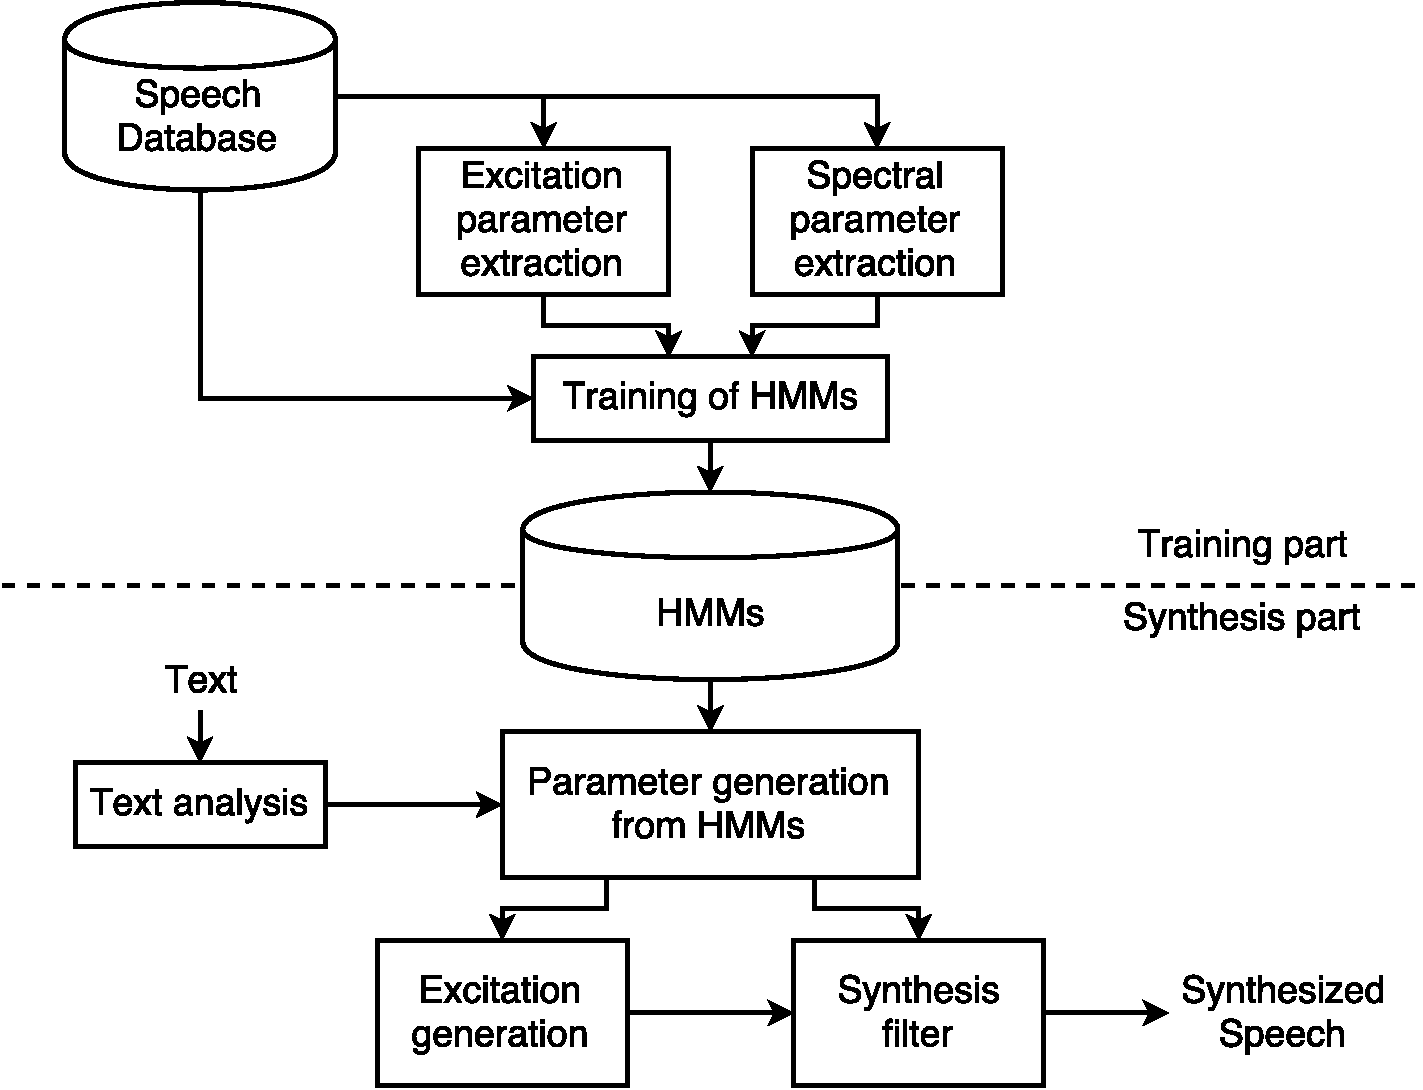
\includegraphics[width=0.8\columnwidth]{hmm-system.pdf}
	\caption{Function blocks of \ac{HMM}-based synthesis \cite{black:statistical}}
	\label{fig:hmm}
\end{figure}

In the synthesis part first the text which is to be synthesized is transformed to a sequence of parameters containing information about the context ({\color{ACMRed}what context?}). According to this sequence the respective \acp{HMM} ({\color{ACMRed}what is that?}) are concatenated in order to form an utterance \ac{HMM}. Then after determining the state durations of the \acp{HMM} a sequence of coefficients is created, which finally is used to construct the speech waveform using a special filter ({\color{ACMRed}details?}).

The main disadvantage of this approach compared to unit-selection synthesis is the quality of the synthesized speech. Three factors are accountable for the lack of quality: the vocoder, the modeling accuracy, and an effect called over-smoothing ({\color{ACMRed}details?}).

However there are some essential advantage, which makes the \ac{HMM}-based approach a competitive alternative to unit-selection synthesis. First, the voice characteristics can be modified without much effort Thus the implementation of different languages and the realization of different speaking styles with emotional emphasize is possible. Second, these just named aspects require a much smaller database than in unit-selection synthesis, since only a statistic representation of speech segments rather than raw speech data is stored. 

In Table~\ref{tab:speechgeneration} the up to here mentioned techniques are compared regarding the most prominent advantages and drawbacks.

\begin{table}[h]
	\caption{Comparison of speech generation methods~\cite{hinterleitner:quality, black:statistical}}
	\label{tab:speechgeneration}
	\begin{tabularx}{1\columnwidth}{cYY}
		\toprule
		\textbf{Technique} & \textbf{Advantages} & \textbf{Drawbacks}\\
		\midrule
		Formant-based & No prerecorded speech required & Very artificial and metallic voice\\
		& & \\[-0.5em]
		Unit-selection & Very high voice quality possible & Large database required\\
		& & \\[-0.5em]
		\ac{HMM}-based & Adjustable voice and small footprint & Voice sounds \ \ muffled\\
		\bottomrule
	\end{tabularx}
\end{table}

%---------------------------------------------------------------------------------
%---------------------------------------------------------------------------------
% SPSS with Deep Learning Models
%---------------------------------------------------------------------------------
%---------------------------------------------------------------------------------

\section{\ac{SPSS} with Deep Learning Models}
\label{sec:deepspeech}

{\color{ACMRed}Although, the approach of \ac{SPSS} has brought many advantages over unit-selection synthesis, as shown in the second chapter, the generated voice is still not as natural as desired. Therefore deep learning models recently have been used to further improve \ac{SPSS}. Since \acp{DNN} have proven to be very effective in speech recognition, they have found their way into speech synthesis. With the use of \acp{DNN} it is possible to represent higher dimensional and correlated features in an efficient way as well as compactly modeling complex mapping functions. Exactly these properties can be used in \ac{SPSS}, where different features representing the context (linguistic, prosody, etc.) have to be considered for the acoustic modeling \cite{hashimoto:effect}.}

{\color{ACMRed}In this section first different approaches of deploying deep learning models are investigated, as shown in \cite{hashimoto:effect} and then one specific approach is explained further, wherefore \cite{zen:deepstatistical} is used as reference.}

\subsection{One specific approach for improvement}
\label{subsec:deepspss}

In the previous section we learned that the quality issue of \ac{HMM}-based speech synthesis is caused by three aspects, the vocoder, the accuracy of acoustic models and the over-smoothing effect. Zen \textit{et al.} \cite{zen:deepstatistical} suggest a specific approach to eliminate one of these causes, the accuracy of acoustic models, by allocating this task to a \ac{DNN}. In conventional \ac{HMM}-based systems the mapping between context features (phonetic and linguistic properties) and speech parameters is done by decision tree based context clustering. Thereby the context-dependent \acp{HMM} are assigned to different clusters depending on the combination of contexts using binary decision trees. Each cluster is characterized by a specific set of speech parameters. In this way it is possible to estimate all \acp{HMM} in a robust way, with a typically sized training database.

However decision trees soon reach their limits when handling complex contexts. Only by increasing the size and in this way decreasing the efficiency of the decision tree more complicated contexts (\textit{e.g.} XOR) can be dealt with. 

In addition to that decision require partitioned input data with each partition having a different set of parameters. In this way whith less data per region overfitting (weak generalization) is likely to happen, which then results in a lack of quality. These downsides can be avoided by using a \ac{DNN} instead of multiple decision trees.

But the use of a \ac{DNN} also introduces two disadvantages: The first one arises in terms of computational power. Both in the training and in the prediction stage decision trees require much less operations (total amount and level of complexity) than \acp{DNN}. The second one has to do with the decision process in its basic form. With decision trees a binary question has to be answered, whilst a \ac{DNN} consists of weighted neurons, which use non-linear activation functions (\textit{e.g.} sigmoid, tanh, ReLU \cite{chung:activation}) to determine their state. As consequence of that interpretable rules are far easier to produce with decision trees, than with \acp{DNN}.

In Figure~\ref{fig:dnnspeech} the structure of a \ac{DNN}-based speech synthesis system is shown. First a sequence of input features is generated after analyzing the input text. These parameters contain numeric values like the number of words in a sentence or the duration of a phoneme as well as binary answers to questions like ''is the current phoneme \textit{aa}?''. Then this parameter sequence is fed into the \ac{DNN} where a mapping to output features is deployed by using forward propagation. The \ac{DNN} has to be trained sometime before with pairs of input and output features from a database. In the following steps the speech parameters are extracted from the statistics of the output features and the voice waveform in turn generated from the speech parameters. this is done in the same way as in the \ac{HMM}-based system. For this system the function blocks of text analysis, parameter generation, and waveform synthesis can be reused from a \ac{HMM}-based system. Only the mapping from input features (\textit{e.g.} linguistic contexts) to output features (spectral and excitation parameters) is implemented in a different way.

\begin{figure}[h]
	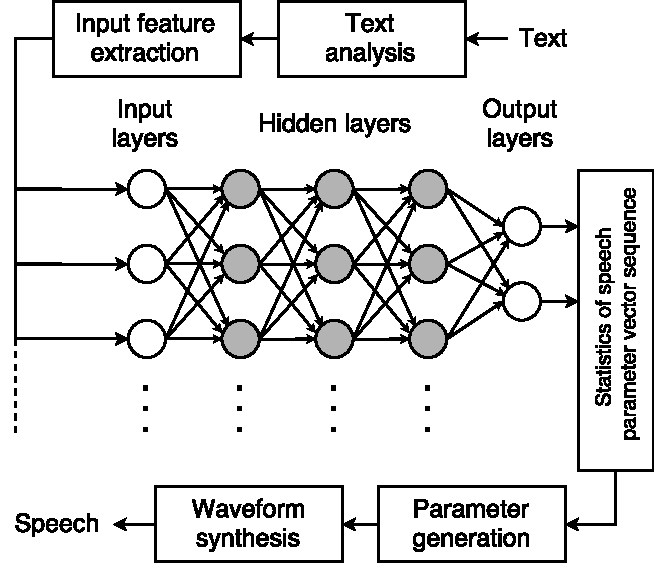
\includegraphics[width=0.8\columnwidth]{dnn-speech-small.pdf}
	\caption{Speech synthesis based on \ac{DNN} \cite{zen:deepstatistical}}
	\label{fig:dnnspeech}
\end{figure}

To compare the output of the above describe framework with that of a \ac{HMM}-based, Zen \textit{et al.} conducted some experiments with each a \ac{HMM}-based and a \ac{DNN}-based speech synthesis system in \cite{zen:deepstatistical}. Therefore they used the same speech data in US English which includes about 33\,000 utterances for both systems. 

The \ac{HMM}-based system used 2\,554 questions for the decision tree-based context clustering. To influence the size of the decision trees the scaling factor $\alpha$ is used, where a high value results in a small decision tree and $\alpha = 1$ denotes a typical \ac{HMM}-based system.

342 binary features (\textit{e.g.} phonemes identities) and 25 numerical features (\textit{e.g.} number of syllables in a word) represent the input features of the \ac{DNN}-based system. As activation function the sigmoid function is used, since the authors experienced superior performance of this type in previous tests. In total one network with different number of layers (1, 2, 3, 4, or 5) and units per layer (256, 1\,024, or 2\,048) are used.

The objective evaluation showed that the \ac{DNN}-based system achieved better performance in voiced/unvoiced classification and aperiodicity prediction, regardless of the number of layers or the units per layer. At the Mel-cepstral distortion only \acp{DNN} with three or more layers outperformed the \ac{HMM}-based system\footnote{\textbf{\color{ACMRed}further explanation}}. 

As subjective evaluation 173 test sentences each synthesized with the \ac{DNN}- and the \ac{HMM}-based systems were played back to a number of listeners, who then choose which synthesis they preferred. If no difference is perceived the option ''neutral'' can be selected. In this test the same number of parameters for both systems are used. For the structure of the \ac{DNN}-based approach 4 layers with a different number of units per layer were applied. In Table~\ref{tab:subeval} the outcome of the subjective evaluation is shown. Unmistakably the speech generated with the \ac{DNN}-based systems were preferred, regardless of the amount of units per layer. The listeners described them as less muffled.

\begin{table}[h]
	\caption{Subjective scores (in \%) of speech samples in~\cite{zen:deepstatistical}}
	\vspace{-0.75em}
	\label{tab:subeval}
	\begin{tabularx}{0.7\columnwidth}{cYc}
		\toprule
		\textbf{\ac{HMM}} & \textbf{\ac{DNN}} & \textbf{Neutral}\\
		($\alpha$) & (layers $\times$ units) & \\
		\midrule
		15.8 (16) & 38.5 (4 $\times$ 256) & 45.7\\[0.5em]
		16.1 (4) & 27.2 (4 $\times$ 512) & 56.8\\[0.5em]
		12.7 (1) & 36.6 (4 $\times$ 1\,024) & 50.7\\
		\bottomrule
	\end{tabularx}
\end{table}

In conclusion it can be stated, that a \ac{DNN}-based approach to implement the acoustic model\footnote{\textbf{\color{ACMRed} other word here???}} of a speech synthesis system is a reasonable alternative to the conventional decision tree-based strategy. The improved performance for predicting spectral and excitation parameters and the more natural sounding voice both show the potential of the \ac{DNN}-based approach for speech synthesis. However the higher computational costs both at training and prediction stage due to more complex arithmetic operations in the \ac{DNN}-based approach indicate where future work should be focused.

\subsection{Other ways for improvement}
\label{subsec:deepeffect}

The previous section focused on the impact a \ac{DNN} has by representing the acoustic model of a speech synthesis system. However deep learning models can be deployed in other parts of \ac{SPSS} as well. In \cite{hashimoto:effect} different ways on how to implement a \ac{DNN} into a speech synthesis are investigated. Therefore the different parts of a \ac{HMM}-based speech synthesis system once are modeled with a \ac{DNN} and once with the conventional technique and then the results are compared in an objective and a subjective fashion.

Hashimoto \textit{et al.} concentrated on two core components of a speech synthesis system, the acoustic models and the speech generation part. In Figure~\ref{fig:generalspeech} you can see the simplified structure of a speech synthesis system. In the first block the text is analyzed and the contextual features are extracted (A). These are then converted to static and dynamic acoustic features (B) by the acoustic models. The parameter generation block then uses these acoustic features to create speech parameters (C). In the last step the speech waveform is synthesized.

\begin{figure}[h]
	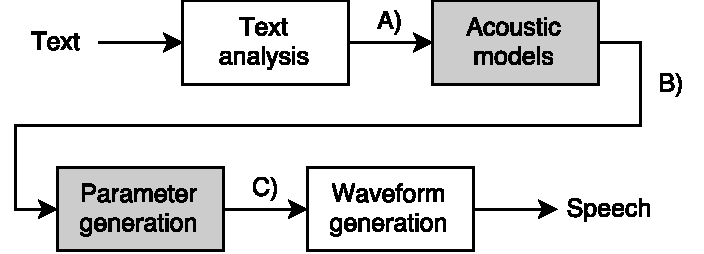
\includegraphics[width=0.8\columnwidth]{speech-general.pdf}
	\caption{Simplified structure of speech synthesis system \cite{hashimoto:effect}}
	\label{fig:generalspeech}
\end{figure}

The two gray-colored blocks in Figure~\ref{fig:generalspeech} are subject of two experiments conducted in \cite{hashimoto:effect}. The conventional approach for the acoustic models is the use of decision tree clustered \acp{HMM}, whereas the parameter generation usually is implemented by a \ac{MLPG} algorithm. As seen in Section~\ref{subsec:deepspss} the acoustic models can be represented by a \ac{DNN}. Hashimoto \textit{et al.} also included this approach in their experiments but furthermore used a \ac{DNN} for the speech parameter generation task.

In Table~\ref{tab:experiments} the systems resulting of the different combinations of the deployment of either conventional or \ac{DNN}-based approach are shown. The systems I~-~IV are part of experiment~1 and all systems except system~IV are part of experiment~2.

\begin{table}[h]
	\caption{Different systems within the experiments \cite{hashimoto:effect}}
	\vspace{-0.75em}
	\label{tab:experiments}
	\centering
	\resizebox{1\columnwidth}{!}{
		\begin{minipage}{\columnwidth}
			\begin{tabularx}{1\linewidth}{X>{\hsize2em}Y>{\hsize2em}Y>{\hsize2em}Y>{\hsize1.75em}Y>{\hsize2.5em}Y>{\hsize2.6em}Y}
				\toprule
				\textbf{System Nr.}& \textbf{I} & \textbf{II} & \textbf{III} & \textbf{IV} & \textbf{V} & \textbf{VI}\\
				\midrule
				Experiments & 1\,\&\,2 & 1\,\&\,2 & 1\,\&\,2 & 1 & 2 & 2\\
				&&&&&&\\[-0.7em]
				Acoustic \ \ \ models & \ac{HMM} & \ac{HMM} & \ac{DNN} & \ac{DNN} & \ac{HMM} & \ac{HMM}\\
				&&&&&&\\[-0.7em]
				Speech \ \ \ \ \ \ \ \ \ \ generation & \ac{MLPG} & \ac{DNN} & \ac{MLPG} & \ac{DNN} & \ac{DNN}~+ \ac{MLPG} & \ac{MLPG} +~\ac{DNN}\\
				\bottomrule
			\end{tabularx}
		\end{minipage}}
\end{table}

In experiment~1 all \acp{DNN} are equipped with three hidden layers and different number of units per layers (256, 512, or 1\,024) and the size of the decision trees was controlled similar as in \cite{zen:deepstatistical}. As objective evaluation only the Mel-cepstral distortion was used. Here the systems with a \ac{DNN} (system~II~-~IV) all outperformed system~I in a similar way, as soon as they had 512 or more units per layer. For the subjective evaluation 20 sentences were played back to 8 listeners who had to assign a naturalness score between 1 and 5 (with 5 being the most natural). After applying the mean opinion score test method, system~III was most preferred with 3.53 followed by system~IV with 3.17 and system~I with 3.08. The less natural sounding voice accoring to the listeners was produced by system~II. From these results it can be concluded, that the speech generation part implemented with \ac{MLPG} (system~I \& III) produces a more natural output than those with a \ac{DNN} (system~II \& IV) \footnote{\textbf{\color{ACMRed}Reasons: parameter trajectories}}.

Due to these outcomes experiment~2 introduces two new test cases, system~V and system~VI. For the parameter generation task a combination of \ac{MLPG} and \ac{DNN} is used, for which the respective input and output features where adapted. Again once an objective and a subjective evaluation like in experiment~1 were conducted. The objective evaluation basically showed the same trend as in experiment~1, as soon as 512 ore more units per layer were used, the Mel-cepstral distortion was less than with the conventional approach (system~I). In the subjective evaluation the two new systems (V~\&~VI) both were preferred over system~I, with system~VI being the most preferred system of this experiment. System~III again was better and system~II again was evaluated less natural than system~I.

As conclusion, we see, that the experiments conducted in \cite{hashimoto:effect} confirmed the results of \cite{zen:deepstatistical}, that the decision tree-clustered \acp{HMM} can be replaced by a \ac{DNN} to improve both the prediction performance as well as the naturalness of the generated speech. Beyond that Hashimoto \textit{et al.} demonstrated, that it is worthwhile to go one step further and deploy an additional \ac{DNN} as post-filtering block into the parameter generation task of the speech synthesis system to even further improve the above named results.

%---------------------------------------------------------------------------------
%---------------------------------------------------------------------------------
% Speech Synthesis on Embedded Devices
%---------------------------------------------------------------------------------
%---------------------------------------------------------------------------------

\section{\ac{TTS} on Mobile Devices}
\label{sec:embeddedspeech}

In this section two approaches to optimize speech synthesis for mobile devices are presented. In the first some optimization steps on a conventional \ac{HMM}-based system are suggested \cite{toth:optimizing} whereas the second approach introduces deep learning models to get rid of the dependence on internet-based services.

\subsection{Motivation and Challenges}
\label{subsec:motembedded}

During the last 10 years, advances in technology have led to a tremendous spread of mobile devices, especially smartphones. According to \cite{statista:smartphones} there are 2.1 billion smartphone users worldwide in 2016 which is forecasted to increase to almost 3 billion in 2020. In \cite{statista:smartphones} it also states, that only in 2016 about 1.5 billion new smartphones were sold. From these numbers we can derive, that already today and with increasing significance in the near future, smartphones constitute an essential part of our daily life.

Especially on smartphones, where the visual output is restricted to a rather small screen, usually not bigger than 5 inch in diagonal, speech enabled interaction can improve the user experience in a significant way. In \cite{toth:optimizing} the following three application scenarios are pointed out: Speech interaction can be used as an extension to existing communication channels, speech can be deployed as main output, if other outputs are restricted (\textit{e.g.} while driving), or speech help visually impaired or blind people to interact with a system at all (\textit{e.g.} screen readers).

However, when implementing a speech synthesis application on a mobile device, the increased computational power and storage capacity on recent smartphones can not be used as in desktop devices. One aspect is the power consumption. An application on a smartphone should use as less processing power as possible to avoid shortening the battery life unnecessarily \cite{toth:optimizing}. Another issue is the restricted amount of main memory (16 - 32 MB RAM per app), which forces each application to be as resource-saving as possible. While accomplishing these demands, the output speech still needs to be processed in real-time, to ensure a good user experience~\cite{boros:robust}.

\subsection{Optimized \ac{HMM}-based Synthesis}
\label{subsec:hmmembedded}

One approach to optimize \ac{HMM}-based speech synthesis for mobile devices can be seen in \cite{toth:optimizing}. Here T\'oth \textit{et al.} conduct a study to optimize a \ac{HMM}-based speech synthesis system in terms of computational power, playback latency and footprint size while ensuring a reasonable quality of the synthesized speech. In the following this approach is explained further.

As already pointed out in Section~\ref{subsec:convenspeech} \ac{HMM}-based speech synthesis offers the best trade-off between speech quality and footprint size. This surely makes it the most appropriate approach to be deployed in mobile systems. T\'oth \textit{et al.} indicate, that there already have been several approaches to optimize \ac{HMM}-based speech synthesis, but they claim to be the first, who emphasize the optimization steps on resource constrained platforms to achieve a reduction in computational costs while still fulfilling real-time responsiveness.

To measure the processing time of the speech synthesis procedure, T\'oth \textit{et al.} divide the \ac{TTS}-process in three steps: The loading of the \ac{HMM} database\footnote{\textbf{\color{ACMRed}explanation}} into main memory (1), the speech parameter generation (2), and the waveform synthesis (3). As test sentence a 17 seconds sequence is chosen, although it is unlikely that such a long utterance has to be synthesized often in real life (since in practice segments with 1~-~5 seconds are synthesized). But in this way it can be ensured, that shorter sequences are likely to be synthesized as desired, if this long sentence can be dealt with adequately.

The following four approaches to optimize \ac{HMM}-based \ac{TTS} are suggested by T\'oth \textit{et al.}:

\begin{enumerate}[label=\arabic*.]		% label=\roman* OR label=\alph* OR label=\arabic*
	\parskip0.25em
	\bfseries
	\item Vocoder parameters
	\item Size of decision trees
	\item Streaming synthesis
	\item Source code optimizations
\end{enumerate}

In the first approach the conventional \ac{MLSA} filter used for speech parameter generation is replaced by a \ac{LSP} filter. In this way the performance in step (2) can be enhanced. Different orders of the \ac{LSP} filter are tested to compare speech subjective quality, with an order of 18 being the conventional setup and 14, 12, and 10 being the optimization approaches.

The second approach dealt with the size of the decision trees. While lowering the number of nodes of a decision tree reduces the quality of synthesized speech, it also decreases the memory footprint and the computational costs. Therefore three different test settings were defined (see Table~\ref{tab:settings}).

\begin{table}[h]
	\caption{Test settings~\cite{toth:optimizing}}
	\vspace{-0.75em}
	\label{tab:settings}
	\begin{tabularx}{1\columnwidth}{lYc}
		\toprule
		\textbf{} & \textbf{Nodes in decision trees} & \textbf{Footprint size}\\
		\midrule
		Original & 6983 & 666 KB\\[0.5em]
		Setting 1 & 4762 & 463 KB\\[0.5em]
		Setting 2 & 2743 & 214 KB\\[0.5em]
		Setting 3 & 1273 & 140 KB\\
		\bottomrule
	\end{tabularx}
\end{table}

General speech synthesis frameworks usually do not include the audio playback functionality to ensure platform independence. Implementing this part allows streaming synthesis. In this way one already synthesized segment is played back while the next segment is generated. While long segments cause an undesired latency, too short segments result in uncontinuous audio playback. The optimal segment size is determined at run-time to achieve a compromise between low as possible latency and low as possible computational effort.

Low-resource devices differ from high-end devices not only in the amount of available memory and the computing performance, but also in the chip architecture. Memory management, fixed- versus floating-point calculation and conditional call management are points to be aware of.

The above described optimizations were tested on three different smartphones with increasing CPU speed and main memory, starting with the ''weakest'': an Apple Iphone 3G, a Samsung Galaxy Spica (GT-i5700) and a HTC Desire (A8181). Therefore the above described optimization steps were tested one by one, since they do not affect each other noteworthy.

For the first approach a \ac{LSP} filter with 12th order was chosen as the optimal setting in terms of latency and subjective speech quality. Concerning the size of the decision trees, setting~1 clearly proved to be the optimal setting, since the time to load the \ac{HMM} database (1) was decreased to half as before without notable impaired speech quality. The streaming synthesis approach tremendously decreased step (1), with an improvement from the order of seconds to 8~ms without affecting the speech quality at all. Concerning the source code optimizations, almost no optimizations have been conducted. Only some conditional calls were removed, which resulted in a insignificant improvement of latency. In total the computation time could be decreased by 65\% without a negligible decrease of speech quality.

\subsection{Deep Learning-based Approach {\color{ACMRed}--- ??? ---}}
\label{subsec:deepembedded}

